\section{Spheremarcher}
\SectionPage


\begin{frame}{Spheremarcher}

    Un \textit{fragment shader} es aplicado a cada píxel de nuestra pantalla, que es procesado por una \textit{hebra} de la \textit{GPU}. \enquote{Lanzararemos un rayo}, de manera numérica, para cada píxel y se aproxima la intersección, de manera iterativa, desde el ojo en la dirección del píxel dirección.
    
    \vfill

    \begin{columns}[onlytextwidth]
        \begin{column}{0.50\textwidth}
            \begin{figure}[H]
              \centering
              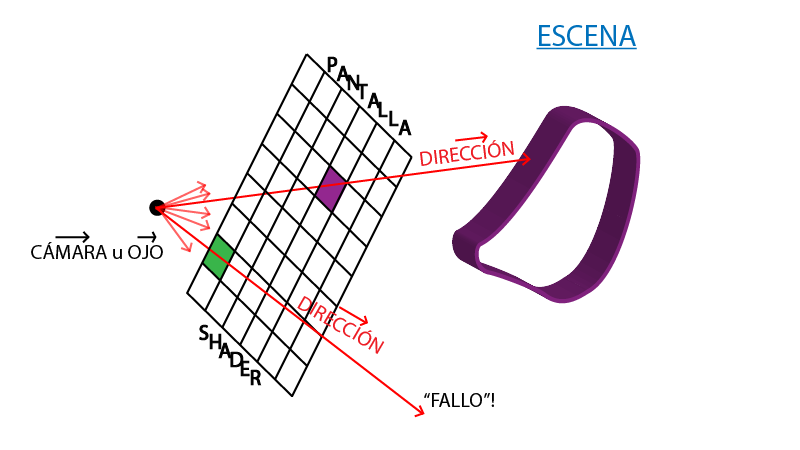
\includegraphics[width=1.0\textwidth]{imagenes/gpu.png}
              %\caption{Fragment shader y Lanzamiento de rayos para el trazado de una escena}
            \end{figure}
        \end{column}
        
        \begin{column}{0.50\textwidth}
            \begin{figure}[H]
              \centering
              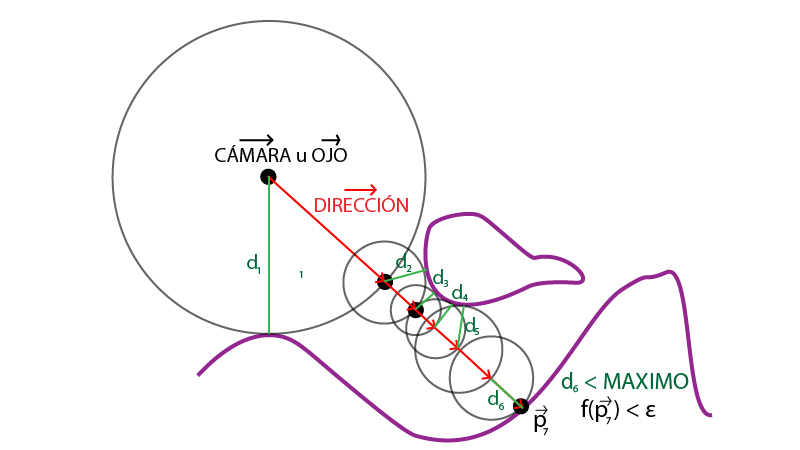
\includegraphics[width=1.0\textwidth]{imagenes/spheremarching.png}
              %\caption{Ejemplo del algoritmo \textit{Spheremarching}}
            \end{figure}
        \end{column}
        
    \end{columns}

\end{frame}


\begin{frame}{Spheremarcher 2}

    Como se ha comentado anteriormente, hacemos uso de las \textit{funciones de distancia con signo} las cuales codifican la escena, \(f:\mathbb{R}^3\longrightarrow\mathbb{R}\). Definimos la posición del \enquote{rayo} en la iteración n-ésima, como:
    \[ \Vec{rayo}_{n}=\Vec{ojo} + \Vec{direccion} \cdot d_{n} \]
    donde \(d_{n}\) es la distancia total recorrida por todas las iteraciones:
    \[d_{n}=d_{n-1} + f(\Vec{p}_{n-1})\text{ con } d_0=0\]
    
    \begin{definition}
        Sea \(f:\mathbb{R}^2\longrightarrow\mathbb{R}\), una función de distancia con signo, definimos como \textit{isoperímetro}, \(L=\{\Vec{p} \vert f(\Vec{p})=0\}\).
    \end{definition}
    
    \begin{definition}
        Sea \(f:\mathbb{R}^3\longrightarrow\mathbb{R}\), una función de distancia con signo, definimos como \textit{isosuperficie}, \(S=\{\Vec{p} \vert f(\Vec{p})=0\}\).
    \end{definition}

\end{frame}

\begin{frame}{Condiciones de parada}
    Al tratarse de un método numérico, vamos a definir las condiciones de parada:
    \vfill
    \begin{enumerate}
        \item \textbf{Primera condición}. Utilizaremos una variable de control, \(\epsilon\) que relajará la restricción de la definición de  \textit{isosuperficie}, haciendo \(f(\Vec{p}_n) < \epsilon\), ya que, si \(\epsilon = 0\), trataríamos de un modelo analítico.
        \item \textbf{Segunda condición}. Superar una cierta distancia recorrida, \(d_{n}\ge MAXIMO\), creando una esfera de trazado sobre el punto de la cámara.
        \item \textbf{Tercera condición}. Superar el número de iteraciones máximas, \(n \ge PASOS\). \textit{PASOS} es una constante fijada.
    \end{enumerate}
    \vfill
    Este algoritmo devolverá \(d_n\), cuando el algoritmo finaliza debido a la \textbf{segunda o tercera condición}, devolverá, \(d_n=MAXIMO\), recibiendo el nombre de \enquote{\textit{fallo}}. Un fallo, representando un pixel vacío, sin superficie trazada, pudiéndose considerar el fondo de la escena.
    
\end{frame}